\section{ДЕМОНСТРАЦИЯ И ТЕСТЫ ПРОИЗВОДИТЕЛЬНОСТИ ПРОГРАММНОГО ПРОДУКТА}

\subsection{Сфера применения программного продукта}

Программный продукт может быть использован в промышленности и энергетики для хранения и последующей аналитики временных рядов. Можно определить лучшие микроклиматические условия для работы человека, способствующие повышению эффективности работника, а так же оптимальные параметры оборудования на предприятии для уменьшения износа их деталей и продления срока службы.

Модуль может быть полезен в сфере энергетики для определения пиковых нагрузок на электростанции для оптимизации работы технических систем. Важно уметь быстро устранять неисправности оборудования, применять горячее или холодное резервирование, чтобы повысить отказоустойчивость электростанции. Не менее важно регулярно проводить техническое обслуживание техники для предовтращения аварий, этого можно достичь с помощью предиктивной аналитики временных рядов параметров технических систем. Всё это может существенно снизить расходы на обслуживание, тем самым снижая стоимость электричества.

Так же модуль может быть использован для аналитики в финансовой сфере. Успех инвестиций напрямую зависит от курса валюты или акции, который можно проанализировать как временной ряд. В сфере телекоммуникаций можно анализировать трафик в сети как временной ряд для оптимизации работы в пиковое время, когда абоненты одновременно загружают сеть.

\subsection{Демонстрация программного продукта}

Для демонстрации программного продукта используется OpenAPI SwaggerUI~\cite{OpenAPI,swaggerui}, который позволяет отправлять запросы к приложению. Пользовательский интерфейс описан в YAML-файле~\cite{swagger-data-types}, его визуализация изображена на рисунке~\ref{swagger1}. Внизу расположена справочная информация о всех запросах и ответах приложения, пример показан на рисунке~\ref{swagger2}.

\begin{figure}
    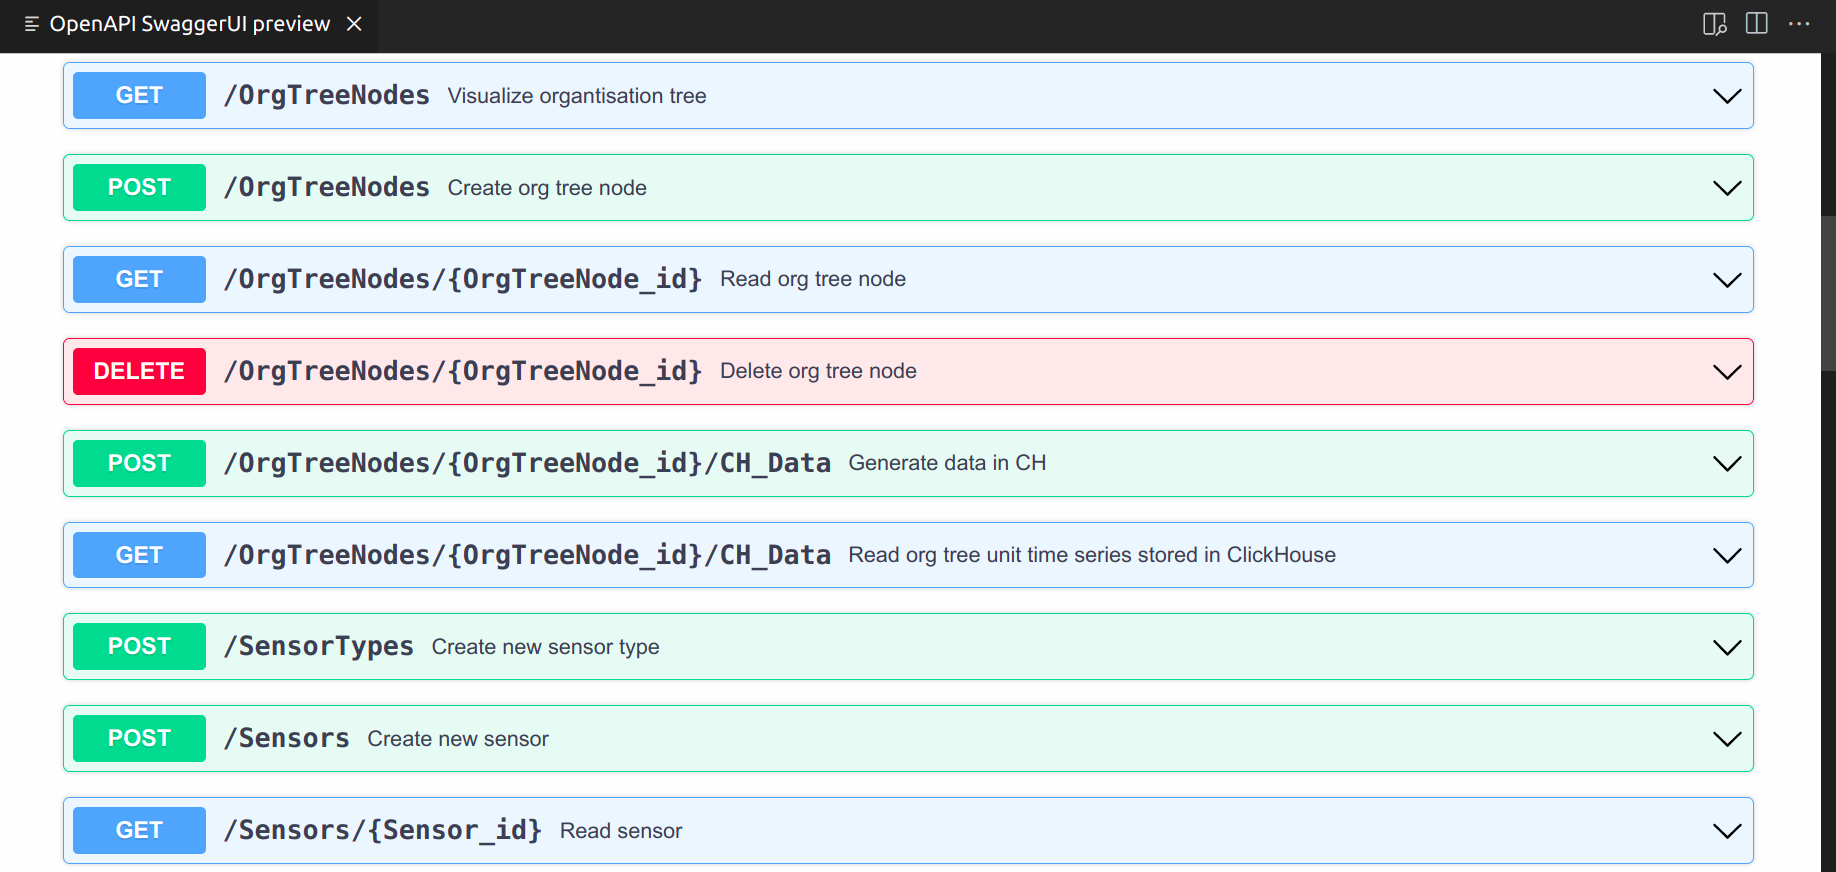
\includegraphics[scale=0.2]{img/swagger1.png}
    \caption{SwaggerUI}
    \label{swagger1}
\end{figure}

\begin{figure}
    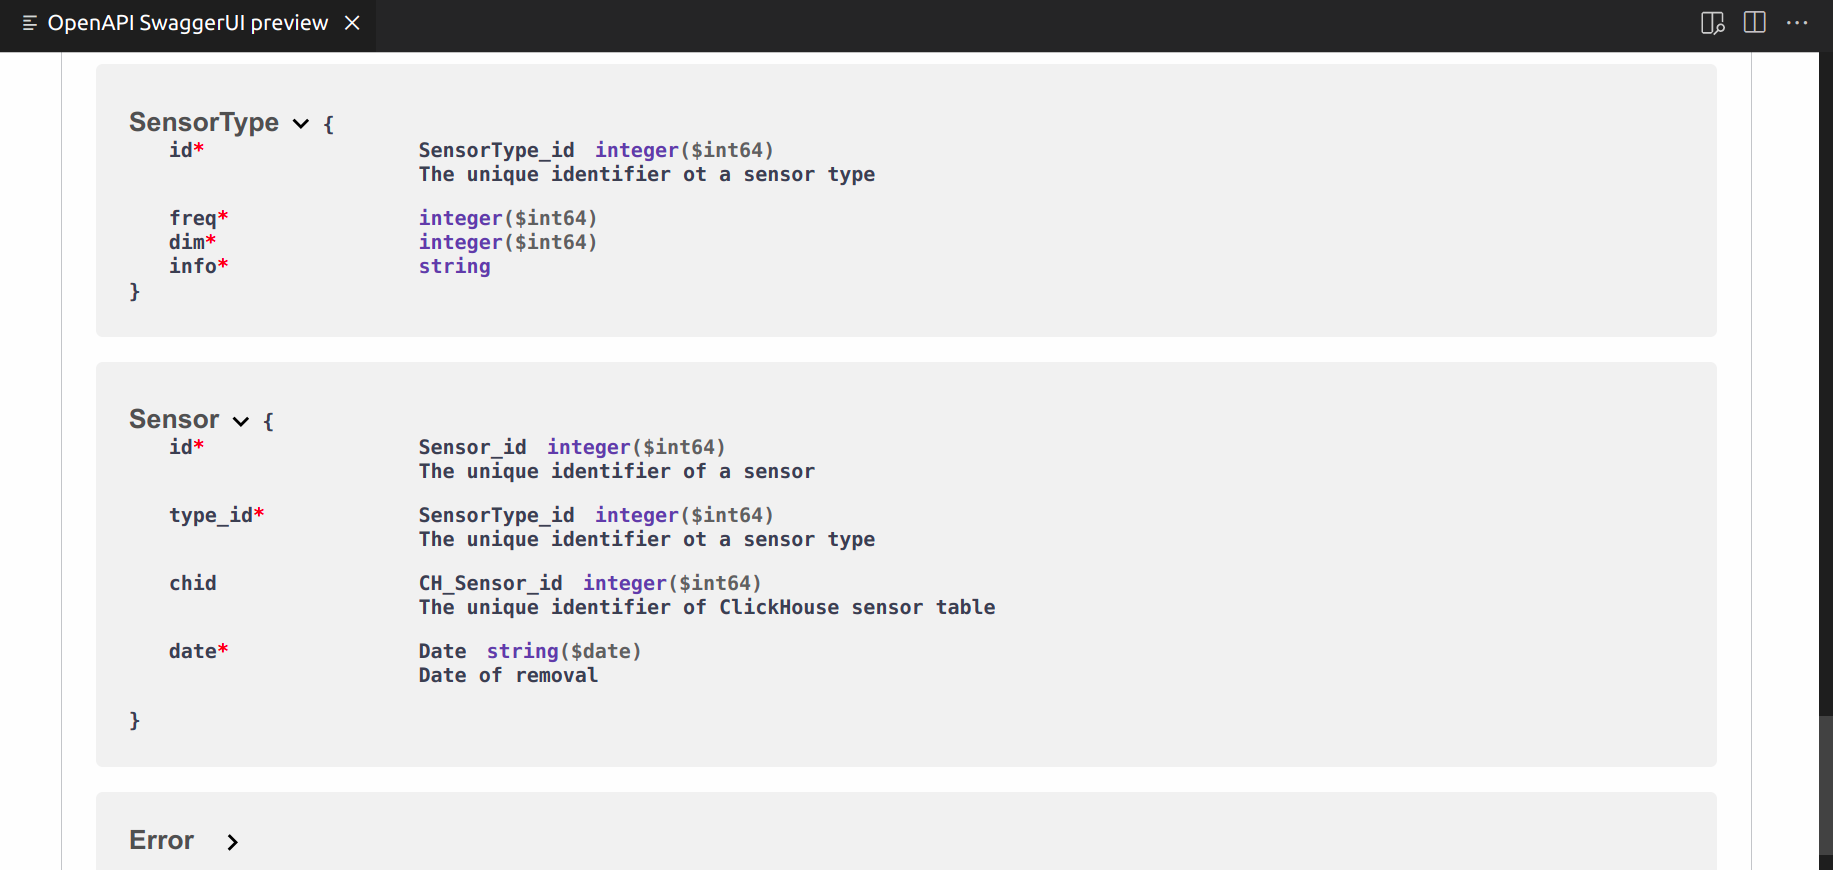
\includegraphics[scale=0.2]{img/swagger2.png}
    \caption{Справочная информация в SwaggerUI}
    \label{swagger2}
\end{figure}

Создадим новую организационную единицу <<My special org unit>>. Это можно сделать, открыв <<POST /OrgUnits>>, как показано на рисунке~\ref{swagger3}. Чтобы создать вершину дерева для этой организационной единицы, необходимо отправить <<POST>> запрос во вкладке <</OrgTreeNodes>> как на рисунке ~\ref{swagger5}. Результаты выполнения запросов приведены на рисунках ~\ref{swagger4} и ~\ref{swagger6} соответственно.

\begin{figure}
    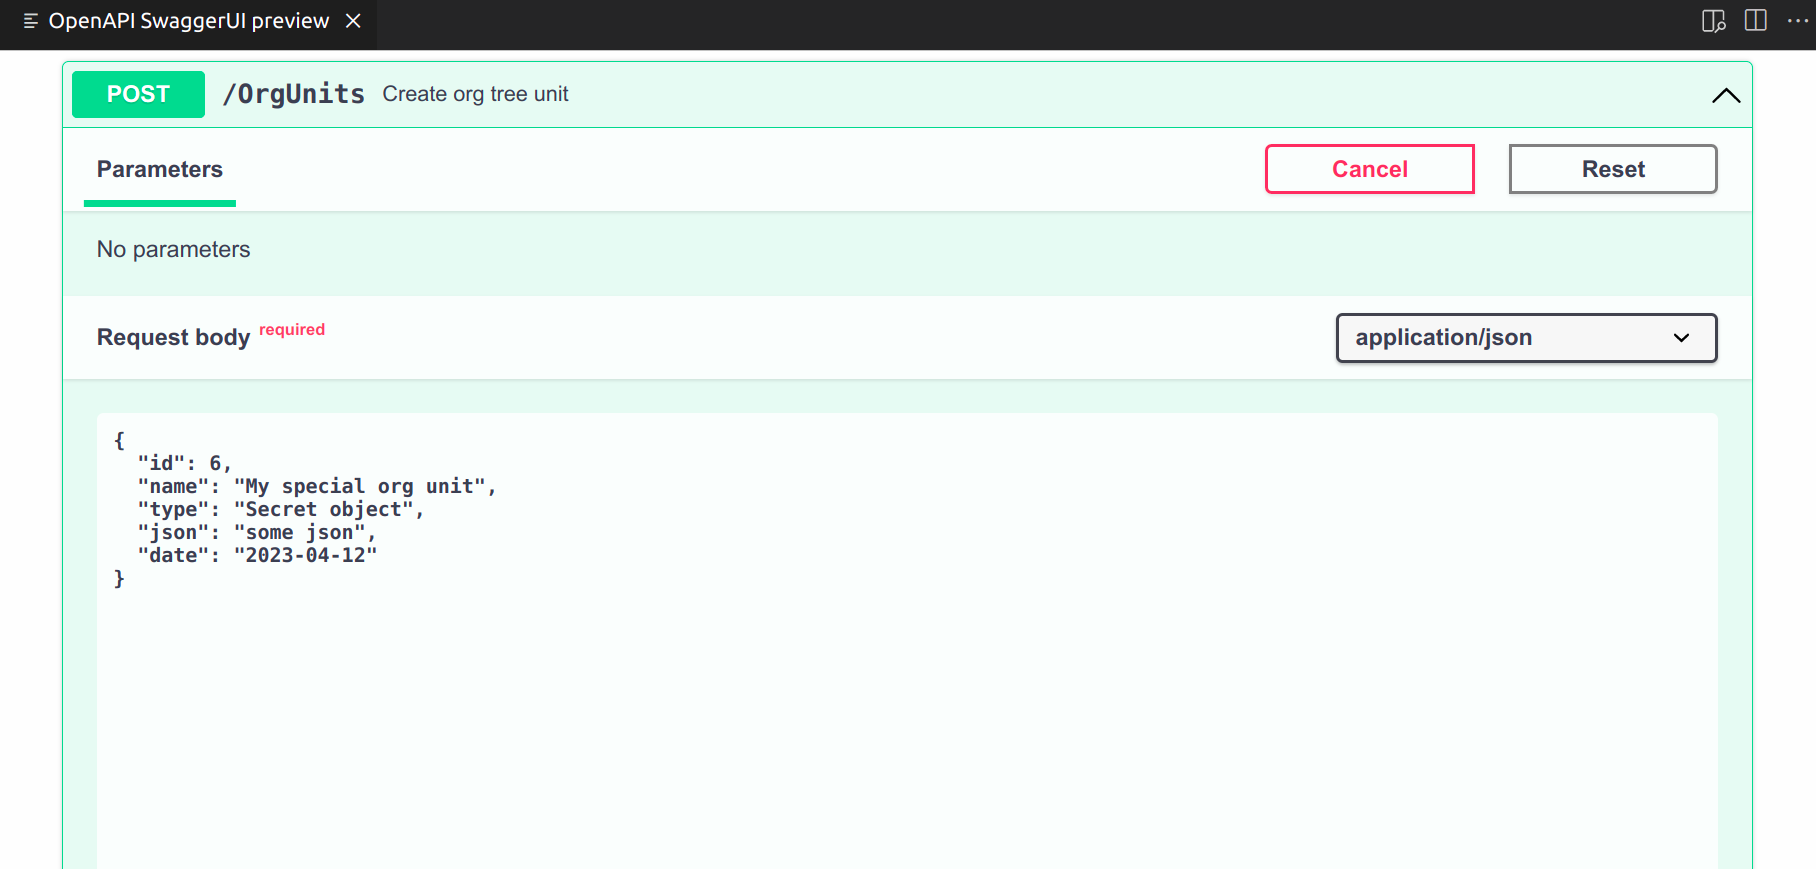
\includegraphics[scale=0.2]{img/swagger3.png}
    \caption{Добавление новой организационной единицы}
    \label{swagger3}
\end{figure}

\begin{figure}
    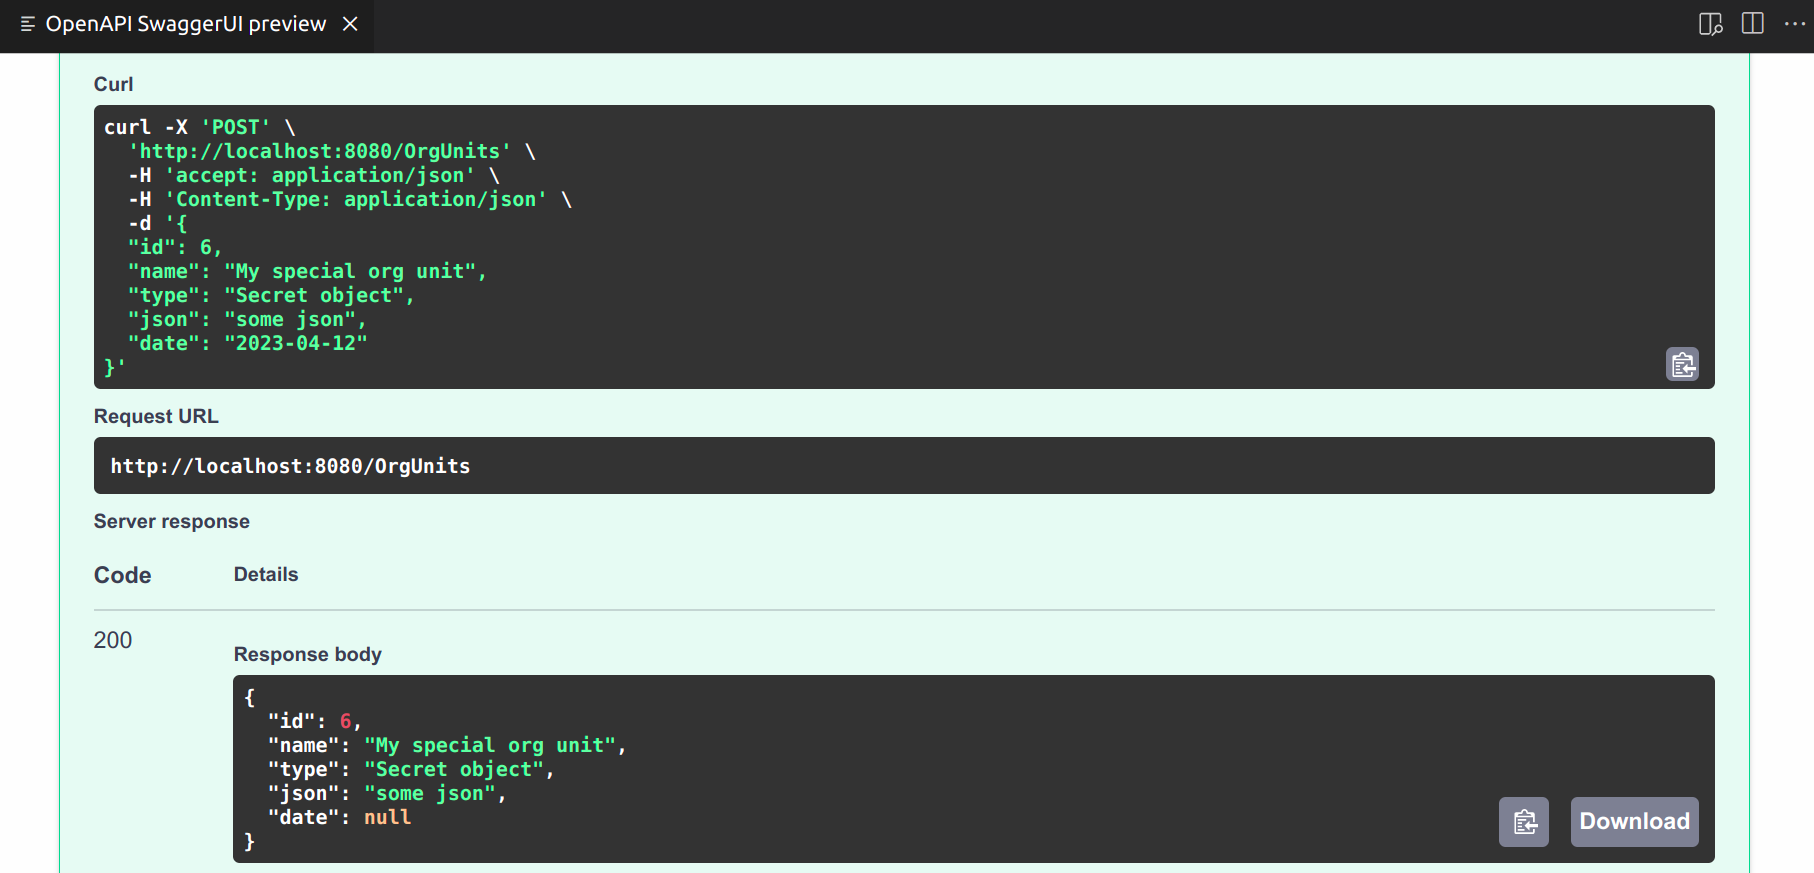
\includegraphics[scale=0.2]{img/swagger4.png}
    \caption{Ответ на запрос добавления организационной единицы}
    \label{swagger4}
\end{figure}

\begin{figure}
    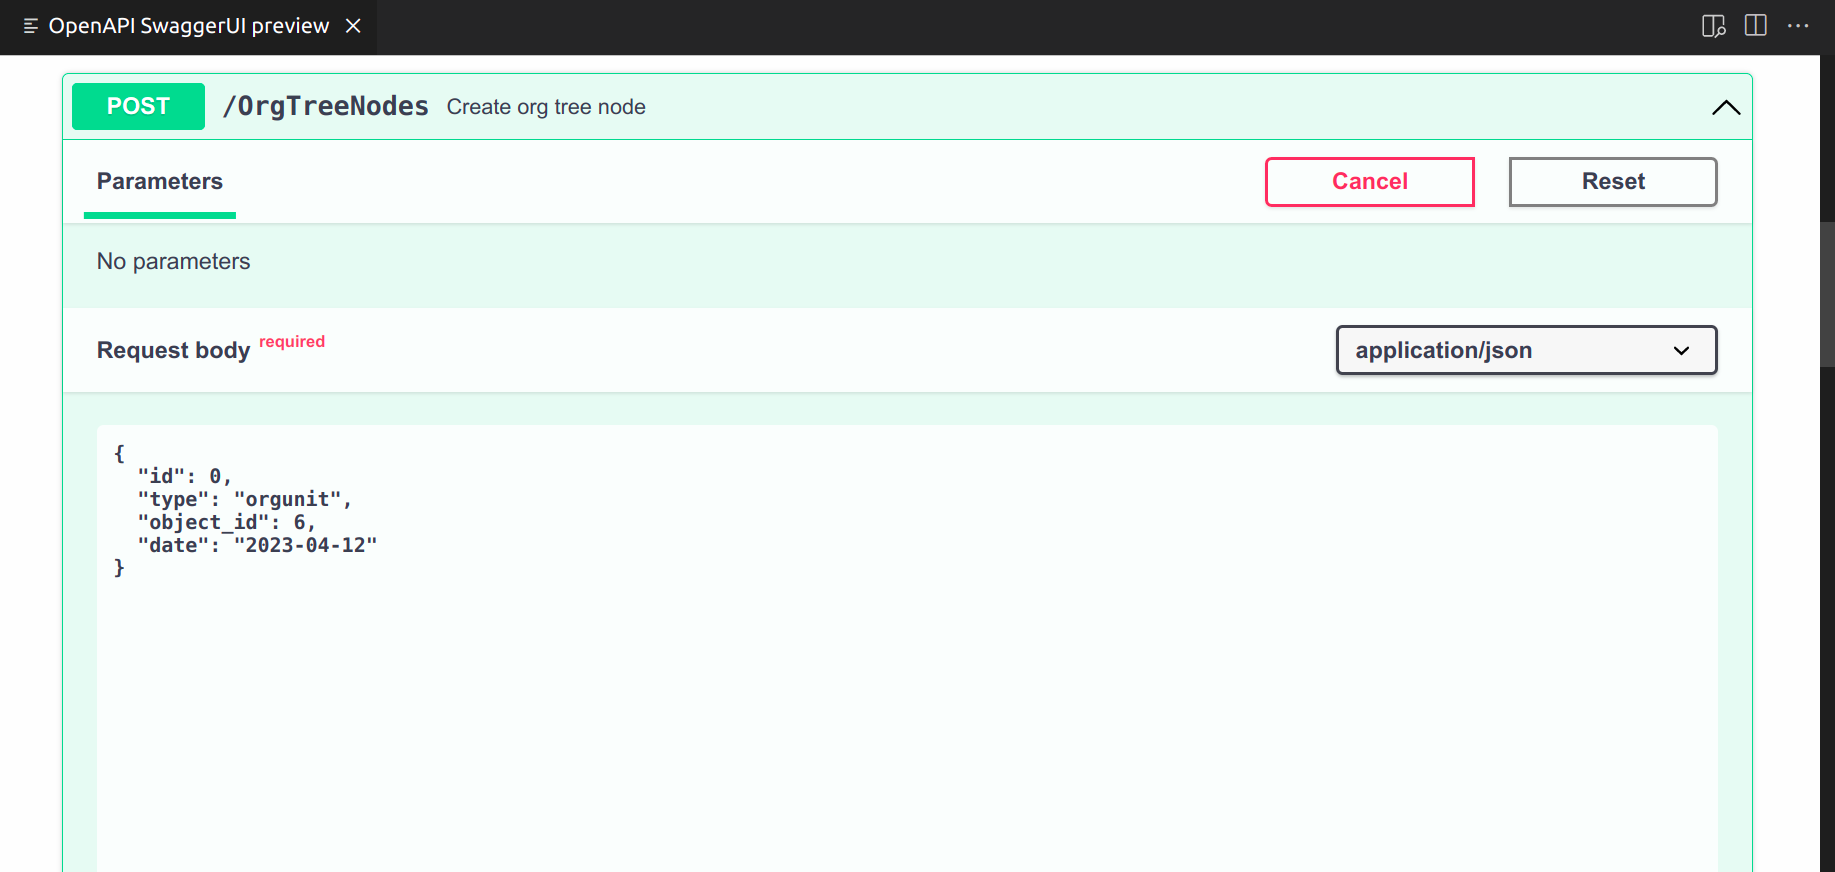
\includegraphics[scale=0.2]{img/swagger5.png}
    \caption{Добавление новой вершины дерева}
    \label{swagger5}
\end{figure}

\begin{figure}
    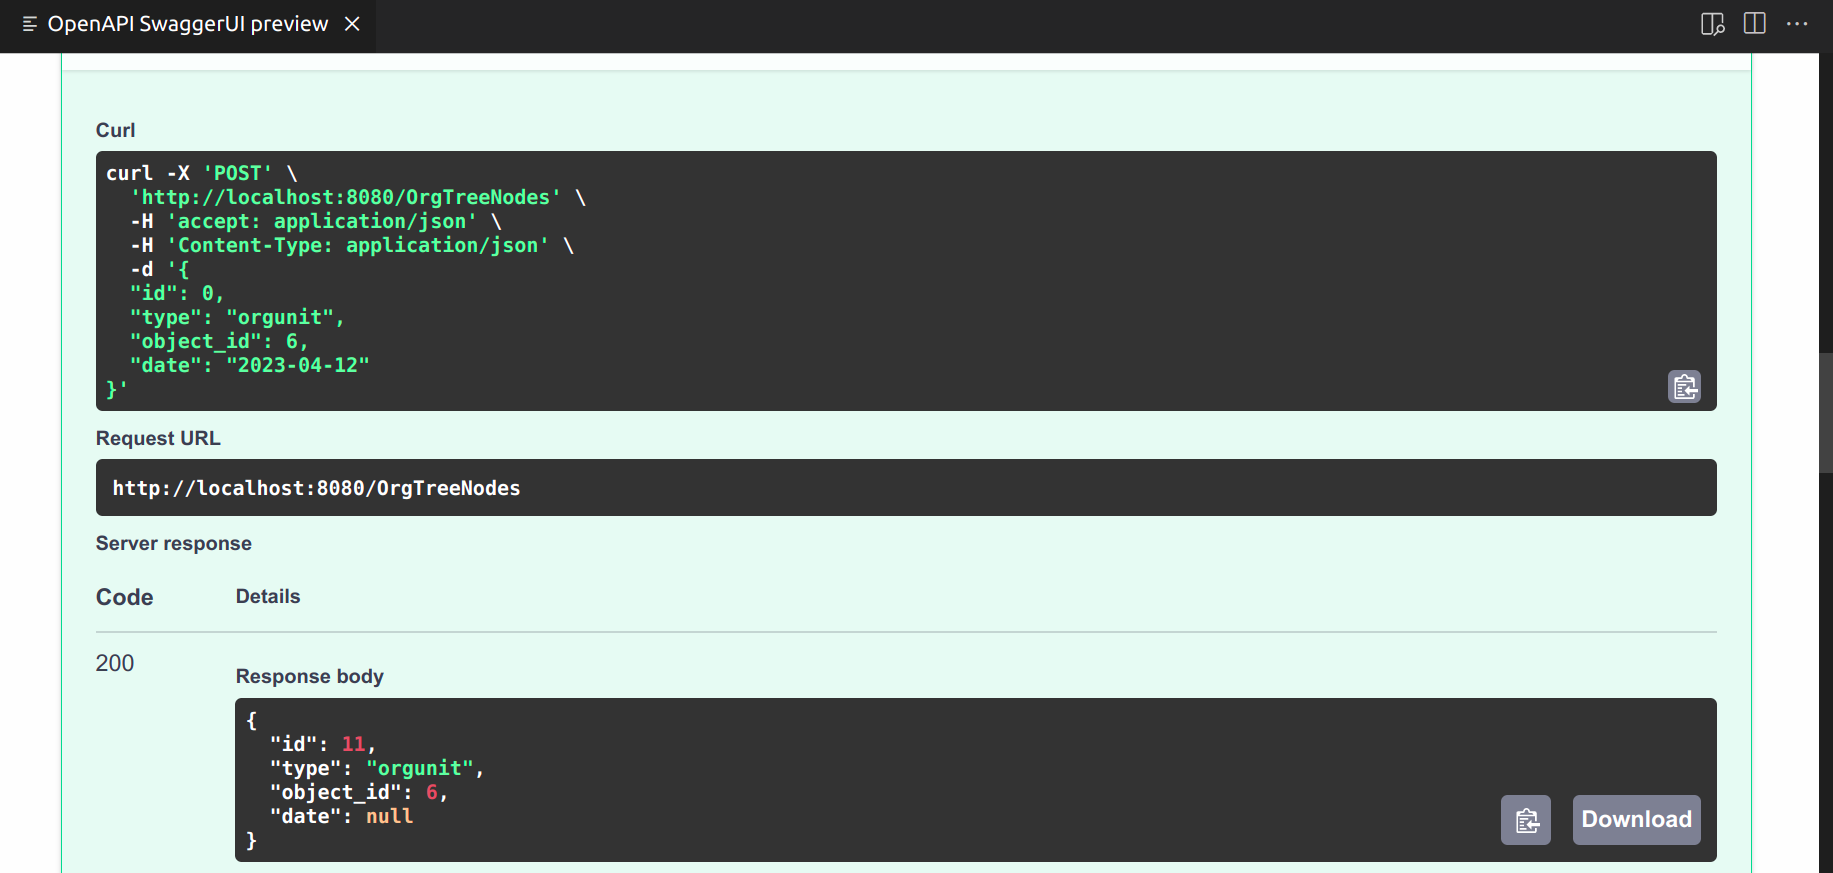
\includegraphics[scale=0.2]{img/swagger6.png}
    \caption{Ответ на запрос добавления вершины дерева}
    \label{swagger6}
\end{figure}

Вкладка <</OrgTreeNodes>> визуализирует текущее дерево организационной структуры. Пример приведён на рисунке~\ref{demo1}. Удалённые вершины и рёбра помечаются пунктирными линиями. После удаления $8$ вершины, всё поддерево с корнем в этой вершине помечается пунктиром, что видно на рисунке~\ref{demo2}.

\begin{figure}
    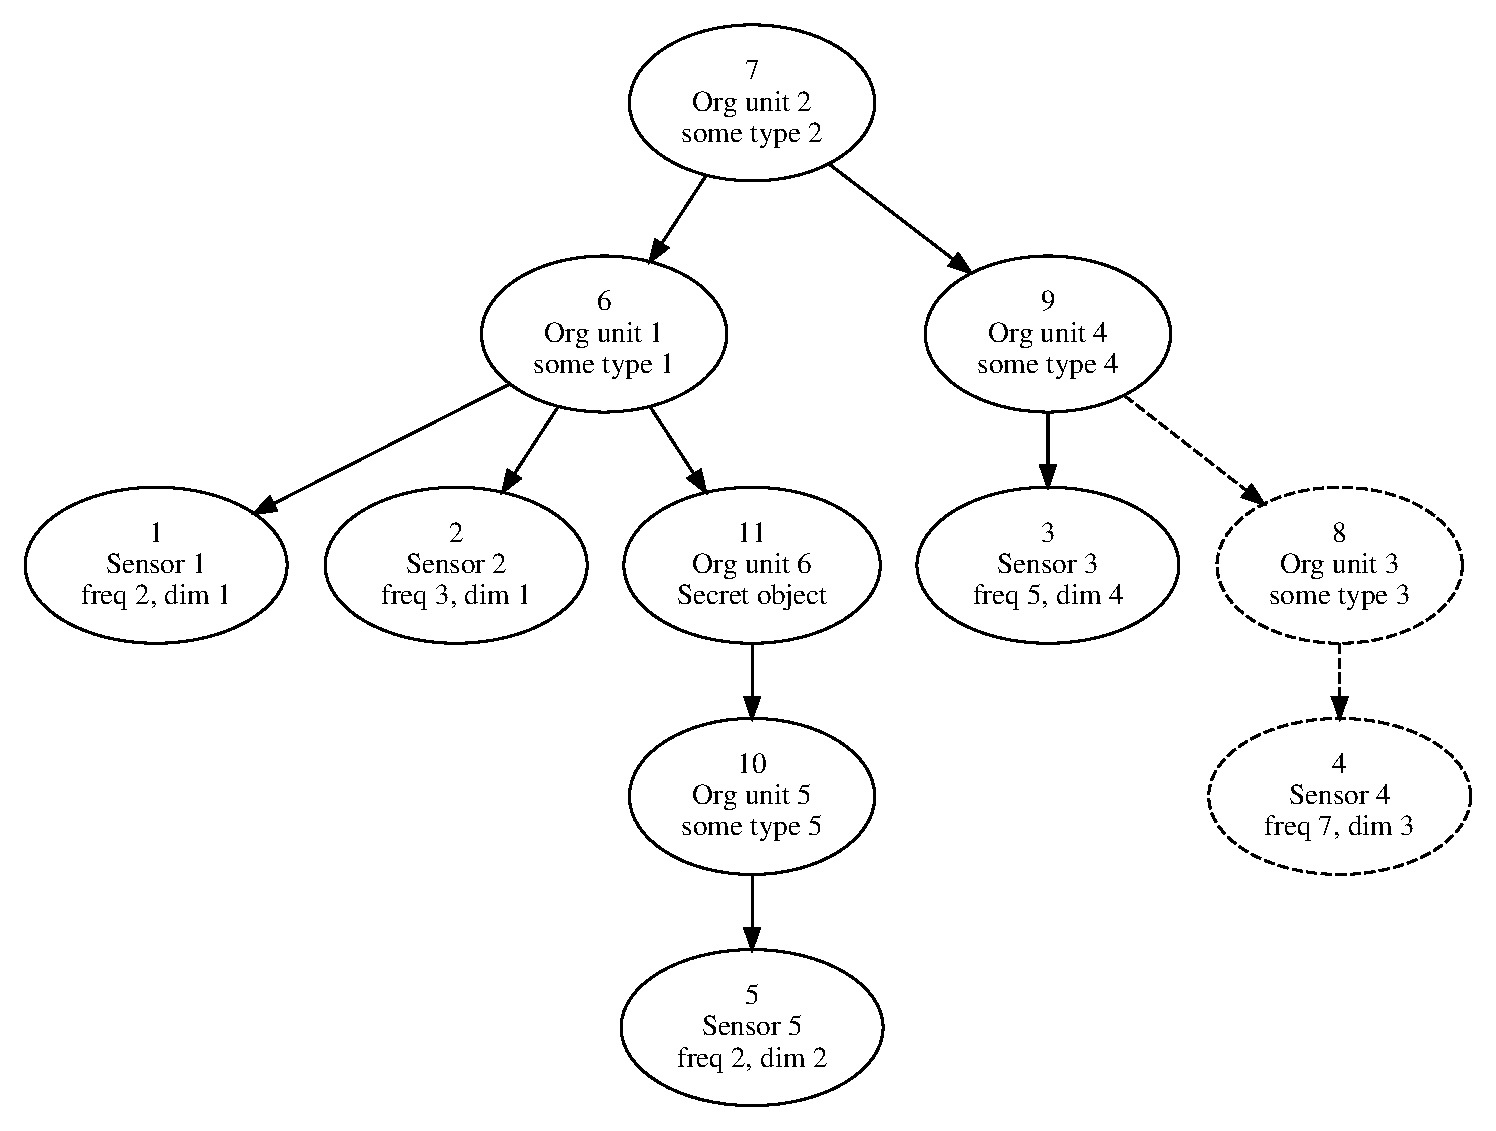
\includegraphics[scale=0.6]{img/demo_del8.eps}
    \caption{Визуализация дерева организационной структуры}
    \label{demo1}
\end{figure}

\begin{figure}
    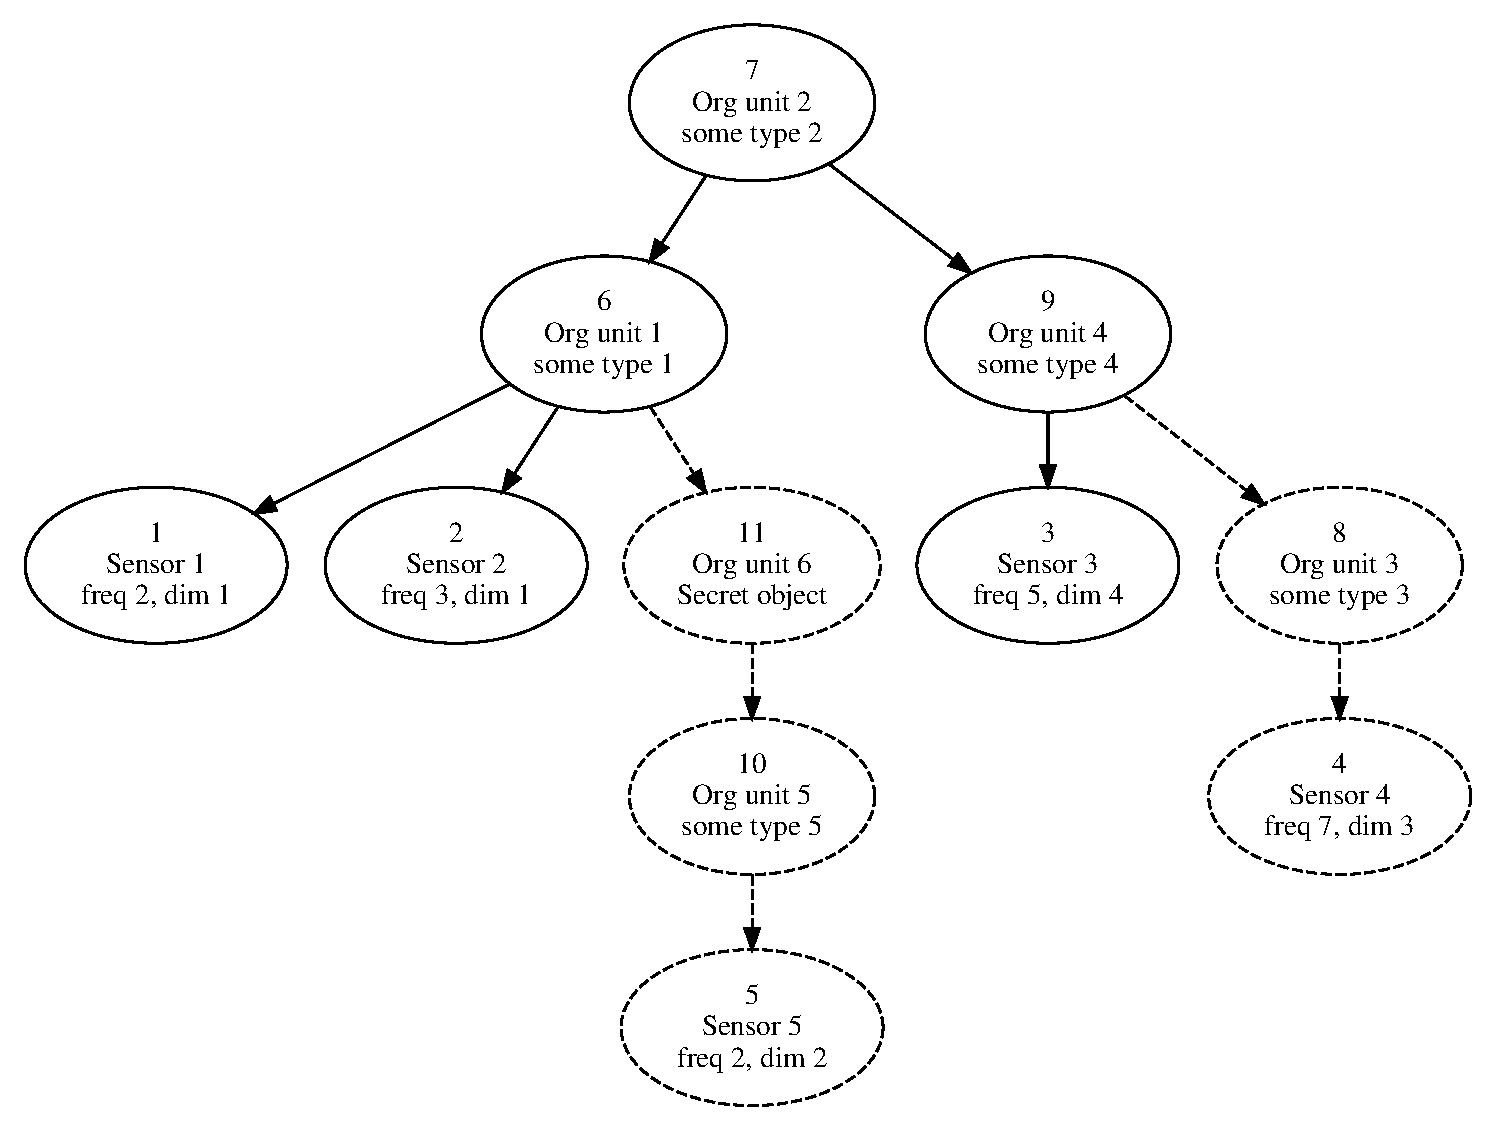
\includegraphics[scale=0.6]{img/demo_del8,11.eps}
    \caption{Визуализация дерева организационной структуры}
    \label{demo2}
\end{figure}

Для получения данных с датчиков необходимо указать номер вершины дерева и промежуток времени, что видно на рисунке~\ref{swagger7}. Результат обработки запроса изображен на рисунке~\ref{swagger8}. После удаления вершины $11$, значит и датчика $5$, данные с него не будут собраны, как показано на рисунке~\ref{swagger9}.

\begin{figure}
    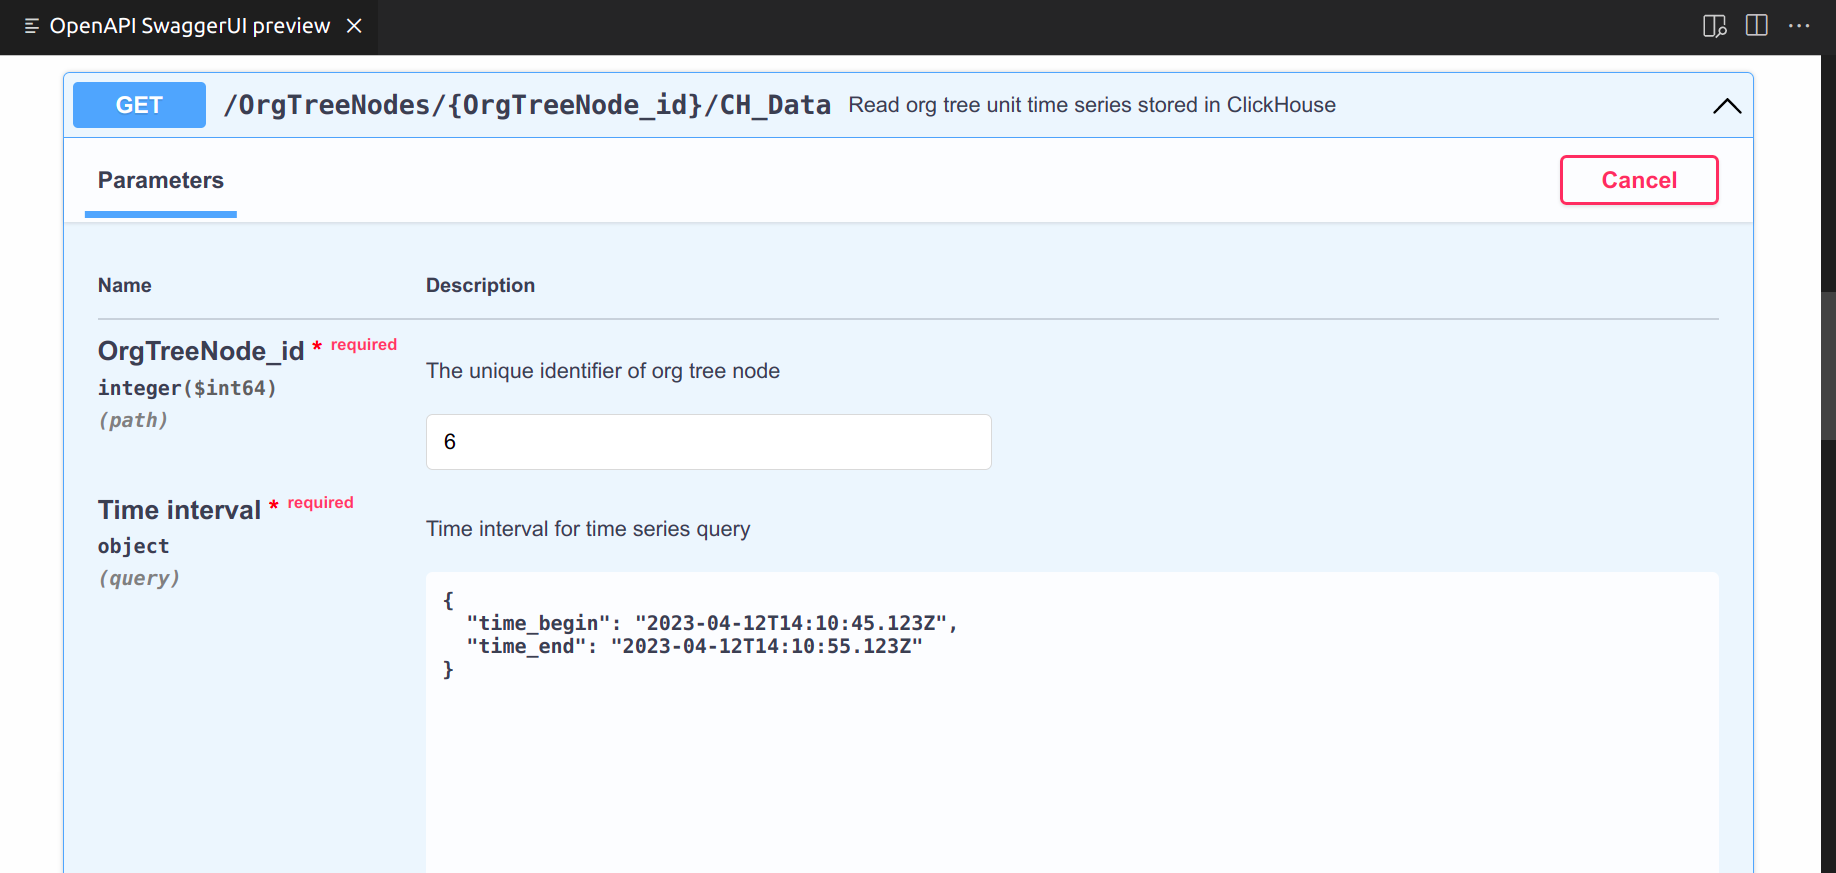
\includegraphics[scale=0.2]{img/swagger7.png}
    \caption{Запрос получения данных с датчиков}
    \label{swagger7}
\end{figure}

\begin{figure}
    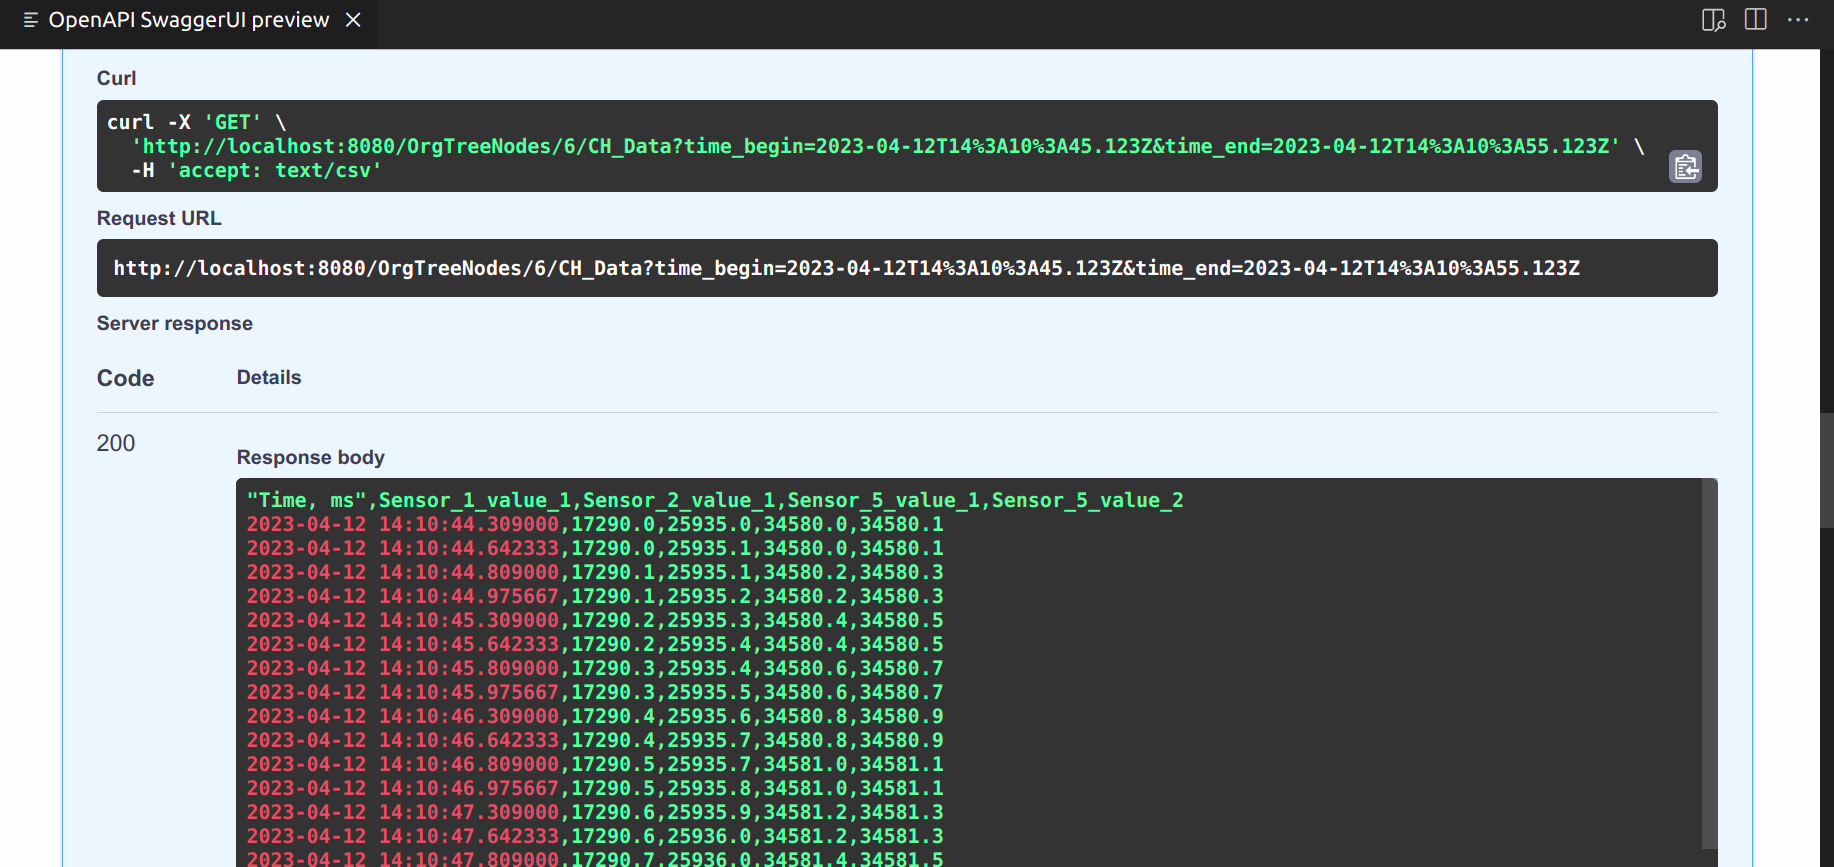
\includegraphics[scale=0.2]{img/swagger8.png}
    \caption{Временные ряды с датчиков $1$, $2$, $5$}
    \label{swagger8}
\end{figure}

\begin{figure}
    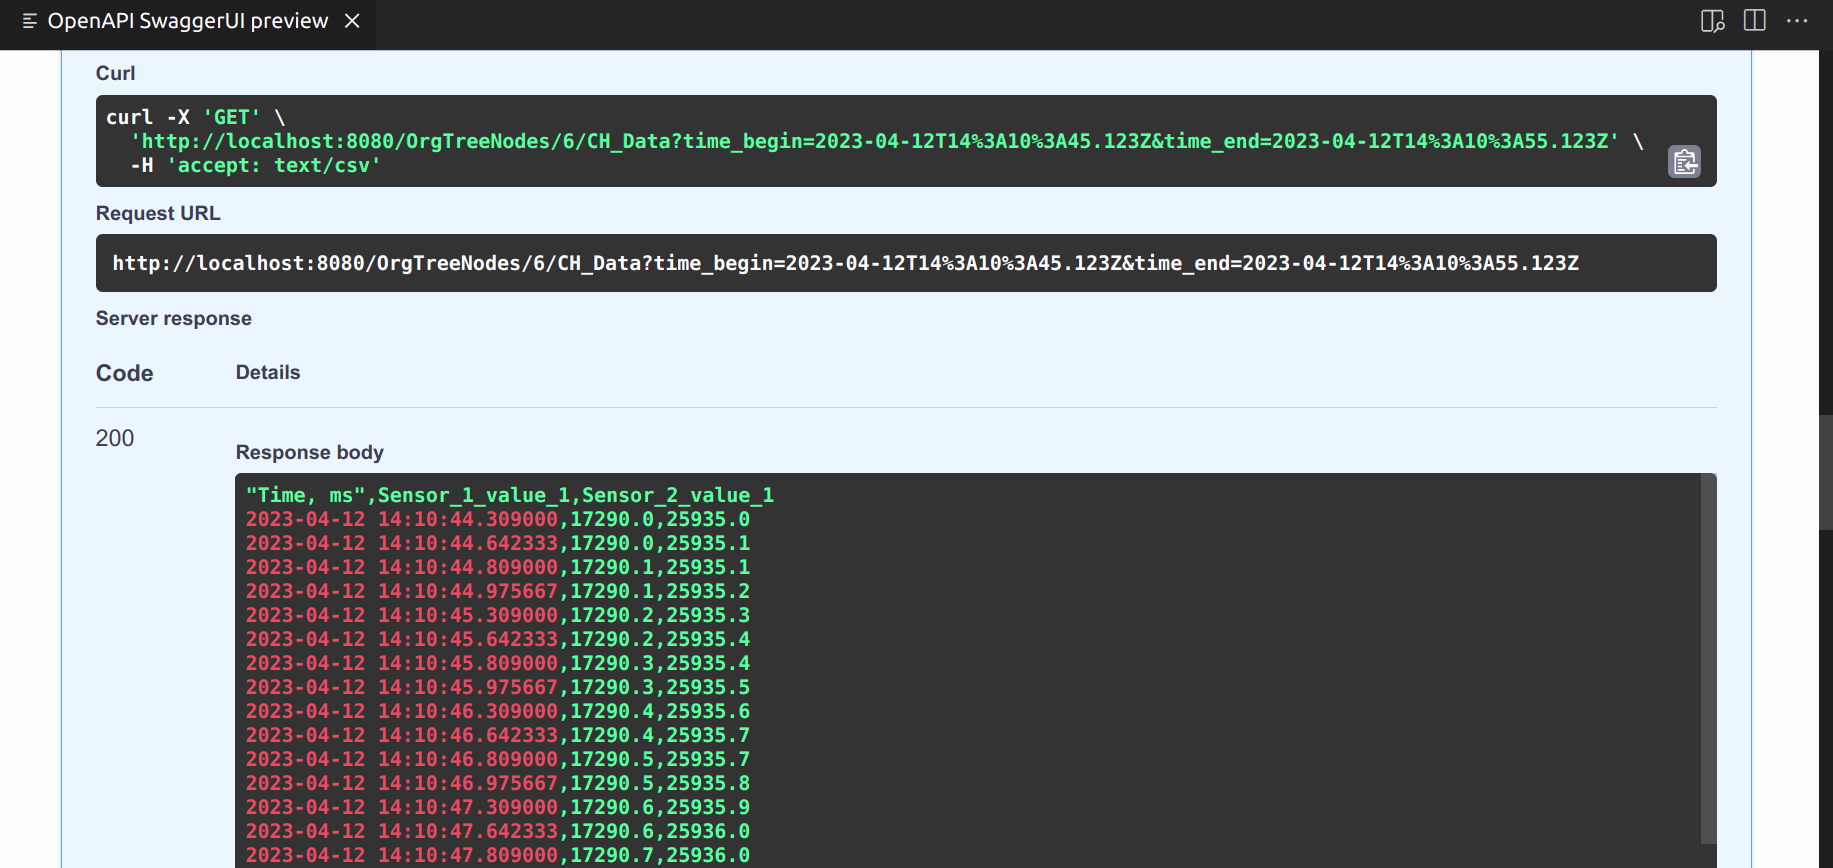
\includegraphics[scale=0.2]{img/swagger9.png}
    \caption{Временные ряды с датчиков $1$, $2$}
    \label{swagger9}
\end{figure}

Данные с датчиков сохраняются в csv таблице~\cite{Python-csv} на диске, так как их может быть очень много. Выше полученные файлы преобразуются в JSON для наглядности~\cite{file-response}.

\subsection{Тесты производительности}

Ранее был приведён алгоритм управления временными рядами, где каждому датчику соответствует отдельная таблица в ClickHouse. Другой подход --- поддерживать одну таблицу для всех датчиков, предварительно выполнив интерполяцию, и отвечать на запрос получения временных рядов, считывая нужные данные.

Для сравнения этих двух подходов в работе генерируются данные и вставляют в таблицы, затем формируются запросы на получение временных рядов датчиков на заданных временных интервалах различной длинны.

Тестирование проводилось на электронной вычислительной машине со следующими техническими характеристиками и программным обеспечением:

\begin{itemize}
    \item центральный процессор <<Intel i7-9750H (12) @ 4.500GHz>>;
    \item оперативная память: два модуля <<Kingston KHX2666C15S4/16G 16384 MB @ 2667MHz>>;
    \item твердотельный накопитель: <<KINGSTON RBUSNS8154P3256GJ (E8FK11.C) 256 GB>>;
    \item операционная система <<Ubuntu 20.04.5 LTS x86\_64>>;
    \item Python 3.8.10;
    \item Docker version 20.10.17, build 100c70180f;
    \item Docker Compose version v2.17.2.
\end{itemize}

Дерево организационной структуры, используемое при тестировании изображено на рисунке~\ref{bench-graph}. Все запросы формируются к вершины под номером $7$, соответствующей организационной единице <<Org unit $2$>>. Таким образом в тесте задействованы датчики под номера $1$, $2$, $3$, $4$ с частотами дискретизации $2$, $3$, $5$ и $7$ соответственно.

\begin{figure}
    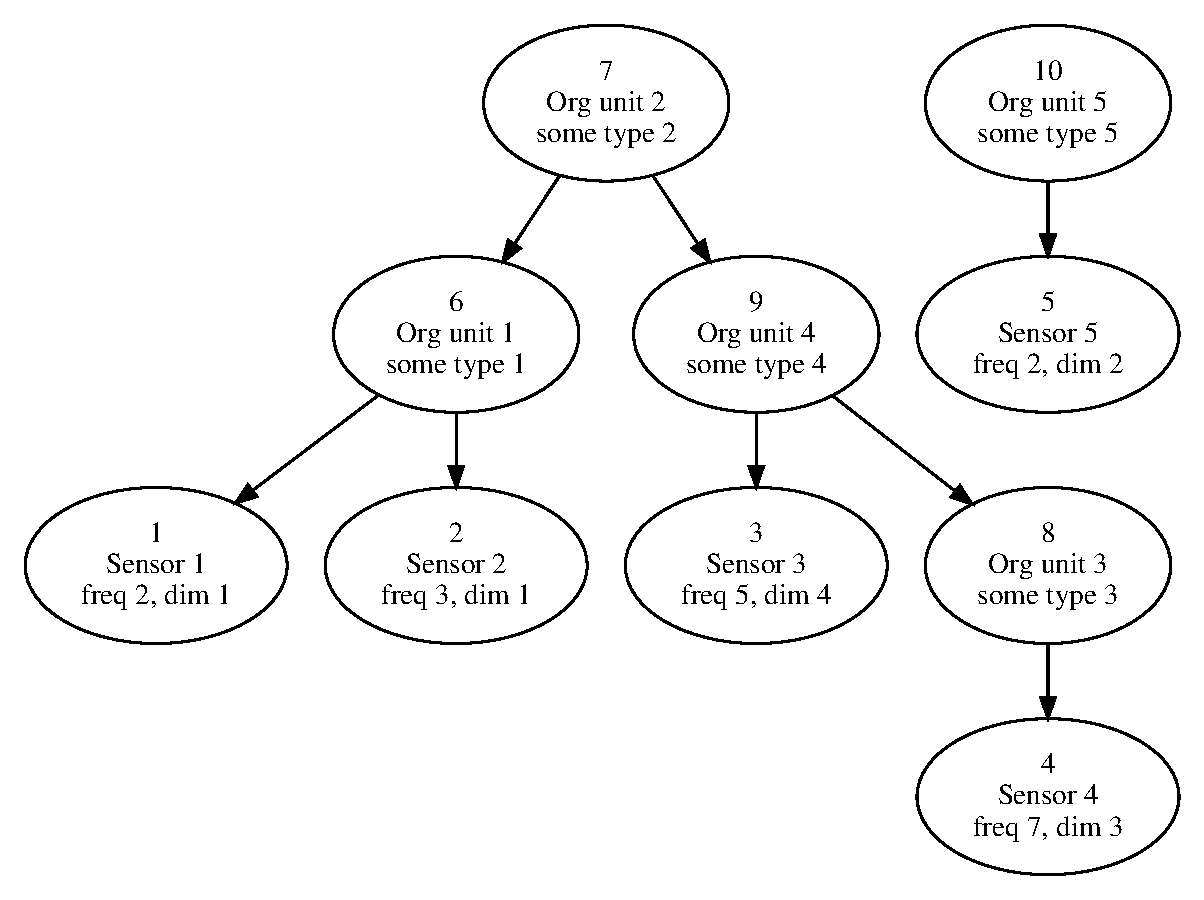
\includegraphics[scale=0.6]{img/bench.eps}
    \caption{Дерево организационной структуры в тесте производительности}
    \label{bench-graph}
\end{figure}

Данные датчиков генерируются на временном интервале $2 \cdot {10} ^ {6}$ секунд. С учётом частот опроса это вставка $3.4 \cdot {10} ^ {7}$ записей в таблицы. Вставка в разные таблицы была выполнена за $155.49$ секунд, а в одну большую таблицу за $262.83$ секунды, так как в ней сразу выполнялась интерполяции значений датчиков.

Для сравнения производительности получения временных рядов были выполнены запросы для временных интервалов длинной $100$, $200$, $500$, $1000$, $2000$, $5000$, $10000$, $20000$, $50000$, $100000$ и $200000$ секунд. Графики времени обработки запроса для длинн до $20000$ секунд приведены на рисунке~\ref{bench2e4}. Видно, что на интерполяцию значений из нескольких таблиц уходит примерно на $20\%$ больше времени.

\begin{figure}
    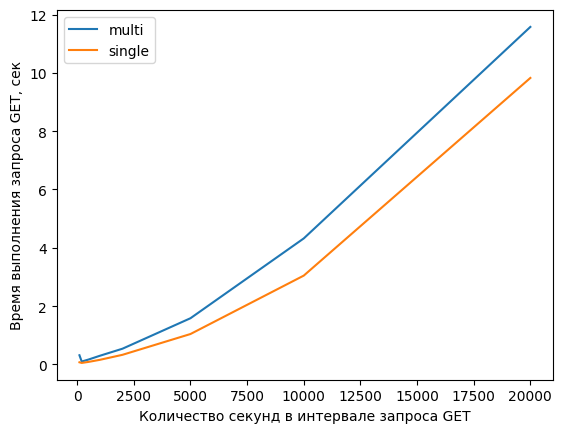
\includegraphics[scale=1.0]{img/bench2e4.png}
    \caption{Графики времени обработки маленьких запросов}
    \label{bench2e4}
\end{figure}

Графики времени обработки запросов для больших временных инервалов приведены на рисунке~\ref{bench2e5}. Интерполяция значений из нескольких таблиц обгоняет и существенно опережает получение данных из одной таблицы. Так как таблицы баз данных хранятся на постоянном запоминающем устройстве компьютера, считывание информации из них занимает больше времени, чем интерполяция в оперативной памяти компьютера. На маленьких временных интервалах затраты на объединение таблиц выше, чем на считывание, однако на больших запросов результат противоположный.

\begin{figure}
    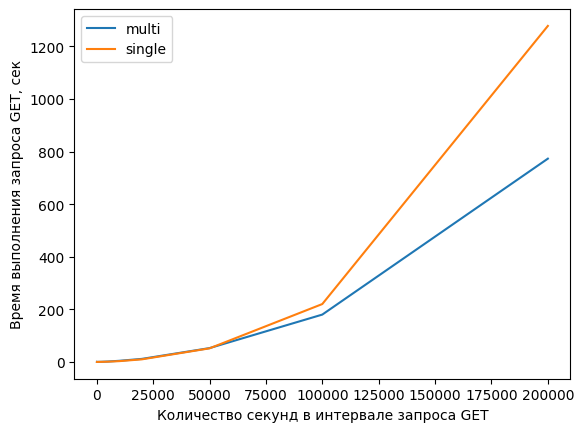
\includegraphics[scale=1.0]{img/bench2e5.png}
    \caption{Графики времени обработки больших запросов}
    \label{bench2e5}
\end{figure}

Из теста производительности следует, что вариант с таблицей под каждый датчик выигрывает по времени у варианта с одной таблицей. Получение временного ряда длительностью $200000$ секунд, что составляет около $3.4 \cdot {10} ^ {6}$ строк в итоговой матрице, заняло $773.06$ секунд.

ClickHouse способен обрабатывать порядка ${10} ^ {6}$ строк в секунду~\cite{ch-perfomance}, поэтому для улучшения производительности программы можно сравнить разные алгоритмы сортировок. Python упрощает разработку динамической типизацией, однако это замедляет программу. Решения на C и C++ обычно быстрее тех, что реализованы на Python, на один-два порядка. При необходимости увеличения производительности время обработки больших запросов может быть сокращено с десяти до пары минут.
